\section{Problem set 1}
\subsection{Problem 1}

\begin{flushleft}
Με $f(x)=e^{-a|x|}$:
\begin{align*}
\mathcal{F}[f(x)]&= \int_{-\infty}^{\infty} f(x) e^{ik x}dx=\int_{-\infty}^{\infty}e^{-a|x|}e^{ik x}dx=\int_{-\infty}^{0} e^{ax}e^{ik x}dx + \int_{0}^{\infty}e^{-ax}e^{ik x} dx\\&= \frac{1}{a+ik}e^{(a+ik)x}\Biggr|_{-\infty}^{0}-\frac{1}{a-ik}e^{-(a-ik)x}\Biggr|_{0}^{\infty}=\frac{1}{a+ik}+\frac{1}{a-ik}=\frac{2a}{a^{2}+k^{2}}
\end{align*}
\end{flushleft}

\begin{figure}[htp]
\centering
\vstretch{1}{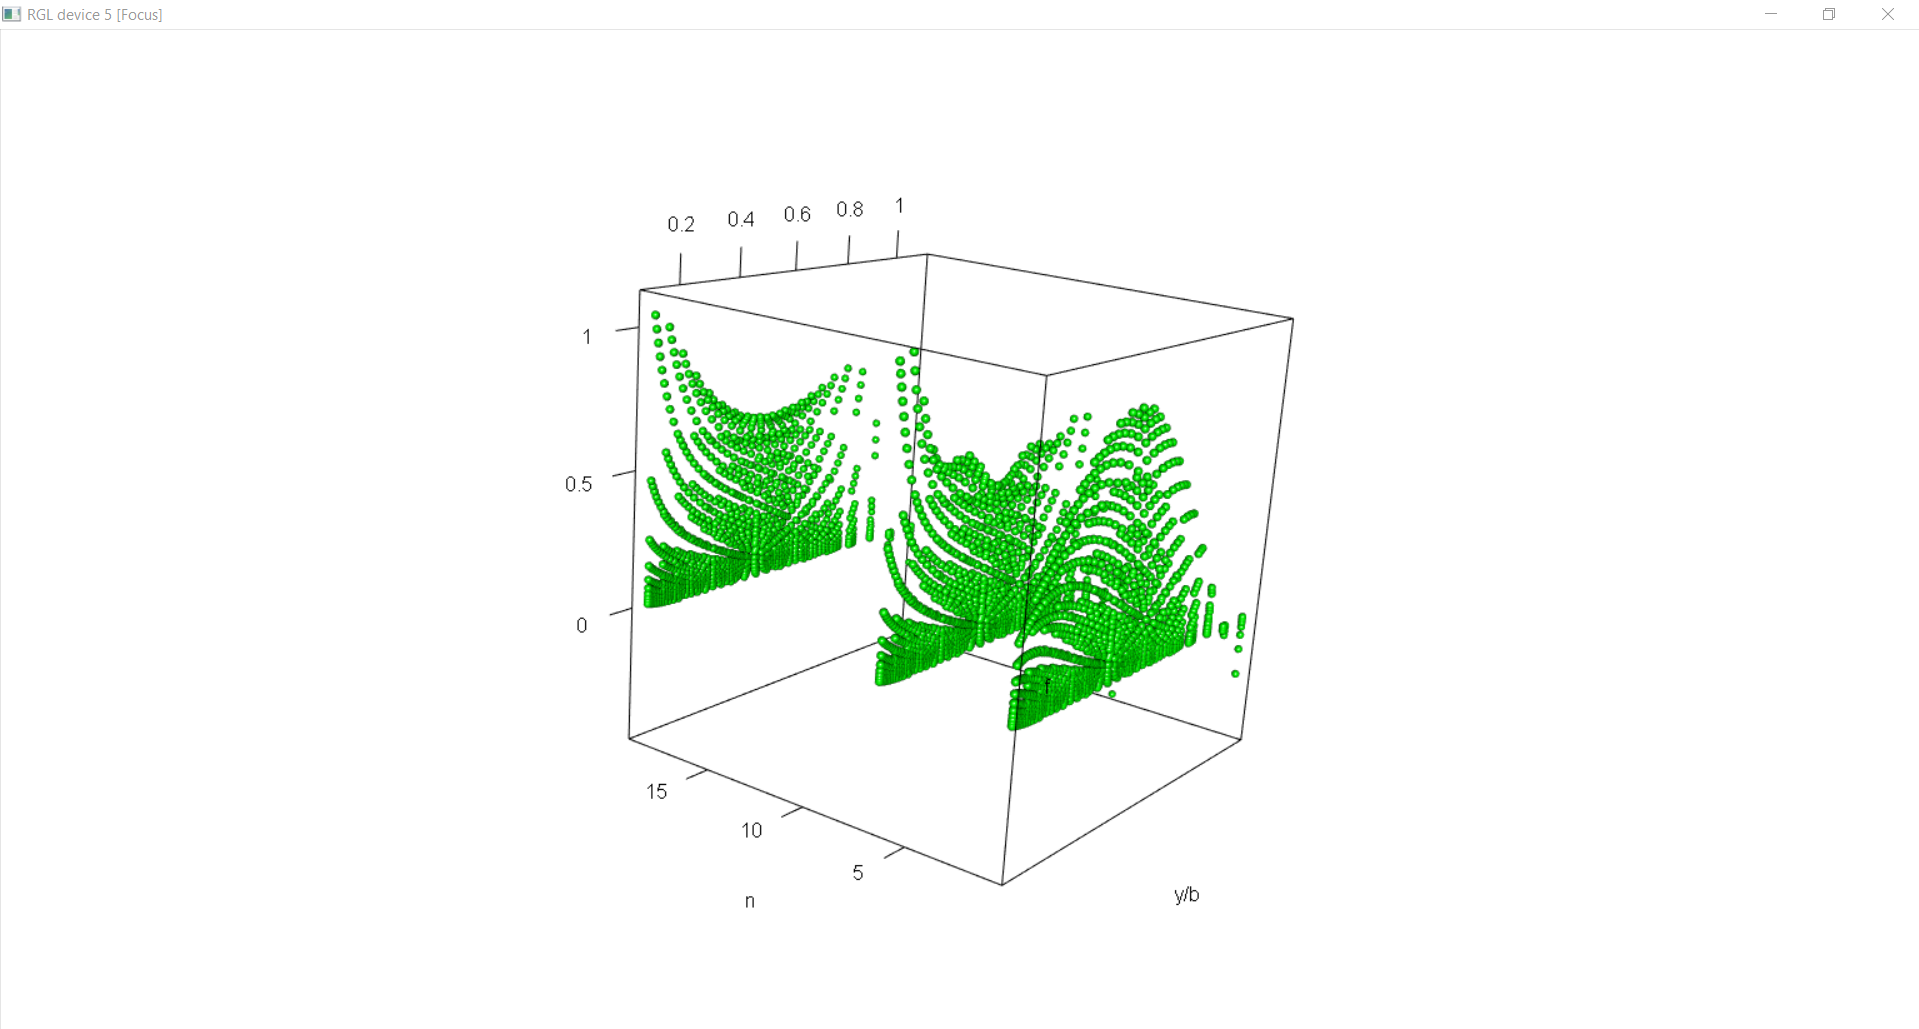
\includegraphics[scale=0.4]{Screenshot_1.jpg}}\caption{FFT στην συνάρτηση $f(x)=e^{-a|x|}$}\label{fig:1}
\end{figure}


\newpage

\begin{figure}[htp]
\centering
\vstretch{1}{\includegraphics[scale=0.4]{Screenshot_2.jpg}}\caption{Στο αριστερό διάγραμμα γίνεται σύγκριση αναλυτικής με αριθμητικής Fourier transformed συνάρτηση στην συνάρτηση $f(x)=e^{-a|x|}$, ενώ στο δεξί παρατίθεται η ποσοτική διαφορά των δύο αυτών.}\label{fig:2}
\end{figure}
\clearpage


\subsection{Problem 2}

\begin{itemize}
\item 1D

Με $f(x)=e^{-ax^{2}}$ και με τη χρήση του ολοκληρώματος Gauss:
\begin{align*}
\mathcal{F}[f(x)]&= \int_{-\infty}^{\infty} f(x) e^{ik x}dx=\int_{-\infty}^{\infty}e^{-ax^{2}}e^{ik x}dx\\&= \int_{-\infty}^{\infty} e^{-a(x^{2}-i\frac{k}{a}x-\frac{k^{2}}{4a^{2}})}e^{-\frac{k^{2}}{4a}}  dx\\&=e^{-\frac{k^{2}}{4a}}\int_{-\infty}^{\infty} e^{-a(x-i\frac{k}{2a})^{2}}dx \\&=e^{-\frac{k^{2}}{4a}}\int_{-\infty}^{\infty} e^{-ax'}dx '=e^{-\frac{k^{2}}{4a}}\sqrt{\frac{\pi}{a}}
\end{align*}

\newpage

\begin{figure}[htp]
\centering
\vstretch{1}{\includegraphics[scale=0.35]{Screenshot_3.jpg}}\caption{FFT στην συνάρτηση $f(x)=e^{-ax^{2}}$}\label{fig:3}
\end{figure}

\begin{figure}[htp]
\centering
\vstretch{1}{\includegraphics[scale=0.35]{Screenshot_4.jpg}}\caption{Στο αριστερό διάγραμμα γίνεται σύγκριση αναλυτικής με αριθμητικής Fourier transformed συνάρτηση στην συνάρτηση $f(x)=e^{-ax^{2}}$, ενώ στο δεξί παρατίθεται η ποσοτική διαφορά των δύο αυτών.}\label{fig:4}
\end{figure}

\clearpage

\item 2D

Με $f(x,y)=e^{-a(x^{2}+y^{2})}=f(x)f(y)$ και πάλι με τη χρήση του ολοκληρώματος Gauss:
\begin{align*}
\mathcal{F}[f(x,y)]&=\int_{-\infty}^{\infty}\int_{-\infty}^{\infty}f(x,y)e^{i(k_{x}x+k_{y}y)}dxdy\\&=\int_{-\infty}^{\infty}f(x)e^{ik_{x}x}dx \int_{-\infty}^{\infty}f(y)e^{ik_{y}y}dy\\&= e^{-\frac{k_{x}^{2}}{4a}}e^{-\frac{k_{y}^{2}}{4a}}\sqrt{\frac{\pi}{a}}\sqrt{\frac{\pi}{a}}=\frac{\pi}{a}e^{-\frac{1}{4a}(k_{x}^{2}+k_{y}^{2})}
\end{align*}



\begin{figure}[htp]
\centering
\vstretch{1}{\includegraphics[scale=0.45]{Screenshot_6.jpg}}\caption{Στο αριστερό διάγραμμα φαίνεται η αριθμητική Fourier transformed συνάρτηση μέσω FFT στην συνάρτηση $f(x)=e^{-a(x^{2}+y^{2})}$, ενώ στο δεξί διάγραμμα φαίνεται η αναλυτική Fourier transformed συνάρτηση στην συνάρτηση $f(x)=e^{-a(x^{2}+y^{2})}$}\label{fig:6}
\end{figure}

\newpage

\begin{figure}[htp]
\centering
\vstretch{1}{\includegraphics[scale=0.8]{Screenshot_7.jpg}}\caption{ Παρατίθεται η ποσοτική διαφορά της αναλυτικής με την αριθμητική λύση ΜΧ Fourier.}\label{fig:7}
\end{figure}



\end{itemize}



\subsection{Problem 3}

Σημείωση: ο ορισμός της κανονικοποιημένης συνάρτησης $\sinc(x)\equiv \frac{sin(\pi x)}{\pi x}$, ενώ ο ορισμός της μή κανονικοποιημένης είναι $sinc(x)\equiv \frac{sin(x)}{x}$. Ενώ στις πράξεις παρακάτω εφαρμόζουμε τον μη κανονικοποιημένο ορισμό, στα Matlab προγραμματάκια χρειάζεται η κανονικοποιημένη συνάρτηση, επομένως η διαφορά των δύο φαίνεται απλώς με έναν μετασχηματισμό $k\rightarrow \frac{k}{\pi}$:
\begin{align*}
\sinc(ka)&=\frac{\sin(ka)}{k}= \frac{\sin(\frac{k}{\pi}a\pi)}{\frac{k}{\pi}\pi}=\frac{\sin(k'a\pi)}{k'\pi}\equiv \sinc_{norm}(k'a)
\end{align*}

\begin{itemize}
\item 1D

Με $f(x)=1$, $x\in [-a,a]$ και $f(x)=0$ αλλού, θα έχουμε:

\begin{align*}
\mathcal{F}[f(x)]&= \int_{-\infty}^{\infty} f(x) e^{ik x}dx = \int_{-a}^{a} e^{ik x}dx =\frac{1}{ik}2i \sin(k a)=\frac{2\sin(k a)}{k}=2a\sinc(ka)
\end{align*}

\newpage

\begin{figure}[htp]
\centering
\vstretch{1}{\includegraphics[scale=0.4]{Screenshot_8.jpg}}\caption{FFT στην συνάρτηση $f(x)=rectangularPulse$ σε 1Δ}\label{fig:8}
\end{figure}

\begin{figure}[htp]
\centering
\vstretch{1}{\includegraphics[scale=0.4]{Screenshot_9.jpg}}\caption{Στο αριστερό διάγραμμα γίνεται σύγκριση αναλυτικής με αριθμητικής Fourier transformed συνάρτηση στην συνάρτηση $f(x)=rectangularPulse$, ενώ στο δεξί παρατίθεται η ποσοτική διαφορά των δύο αυτών.}\label{fig:9}
\end{figure}

\clearpage

\item 2D

Με $f(x,y)=1$, $x\in [-a,a]$,$y\in [-a,a]$ και $f(x,y)=0$ αλλού, θα έχουμε:

\begin{align*}
\mathcal{F}[f(x,y)]&=\int_{-\infty}^{\infty}\int_{-\infty}^{\infty} f(x,y) e^{i(k_{x} x+k_{y} y)}dxdy\\&= \int_{-a}^{a} e^{ik_{x} x}dx \int_{-a}^{a} e^{ik_{y} y}dy\\&= \frac{4}{k_{x}k_{y}} \sin(k_{x}a)\sin(k_{y}a)=4a^{2}\sinc(k_{x}a)\sinc(k_{y}a)
\end{align*}


\begin{figure}[htp]
\centering
\vstretch{1}{\includegraphics[scale=0.7]{Screenshot_10.jpg}}\caption{Η συνάρτηση $f(x,y)=rectangularPulse$ σε 2Δ}\label{fig:10}
\end{figure}

\newpage

\begin{figure}[htp]
\centering
\vstretch{1}{\includegraphics[scale=0.35]{Screenshot_11.jpg}}\caption{Σύγκριση αναλυτικής (δεξιά) με αριθμητικής (αριστερά) Fourier transformed συνάρτηση στην συνάρτηση $f(x,y)=rectangularPulse$ σε 2Δ}\label{fig:11}
\end{figure}



\begin{figure}[htp]
\centering
\vstretch{1}{\includegraphics[scale=0.45]{Screenshot_12.jpg}}\caption{ Σύγκριση αναλυτικής με αριθμητικής Fourier ποσοτικά}\label{fig:12}
\end{figure}
\clearpage

\end{itemize}


